% =============================================================================
% Figure captions for: A Unified Cellular Circuit Model
% =============================================================================

\begin{figure*}[!htbp]
    \centering
    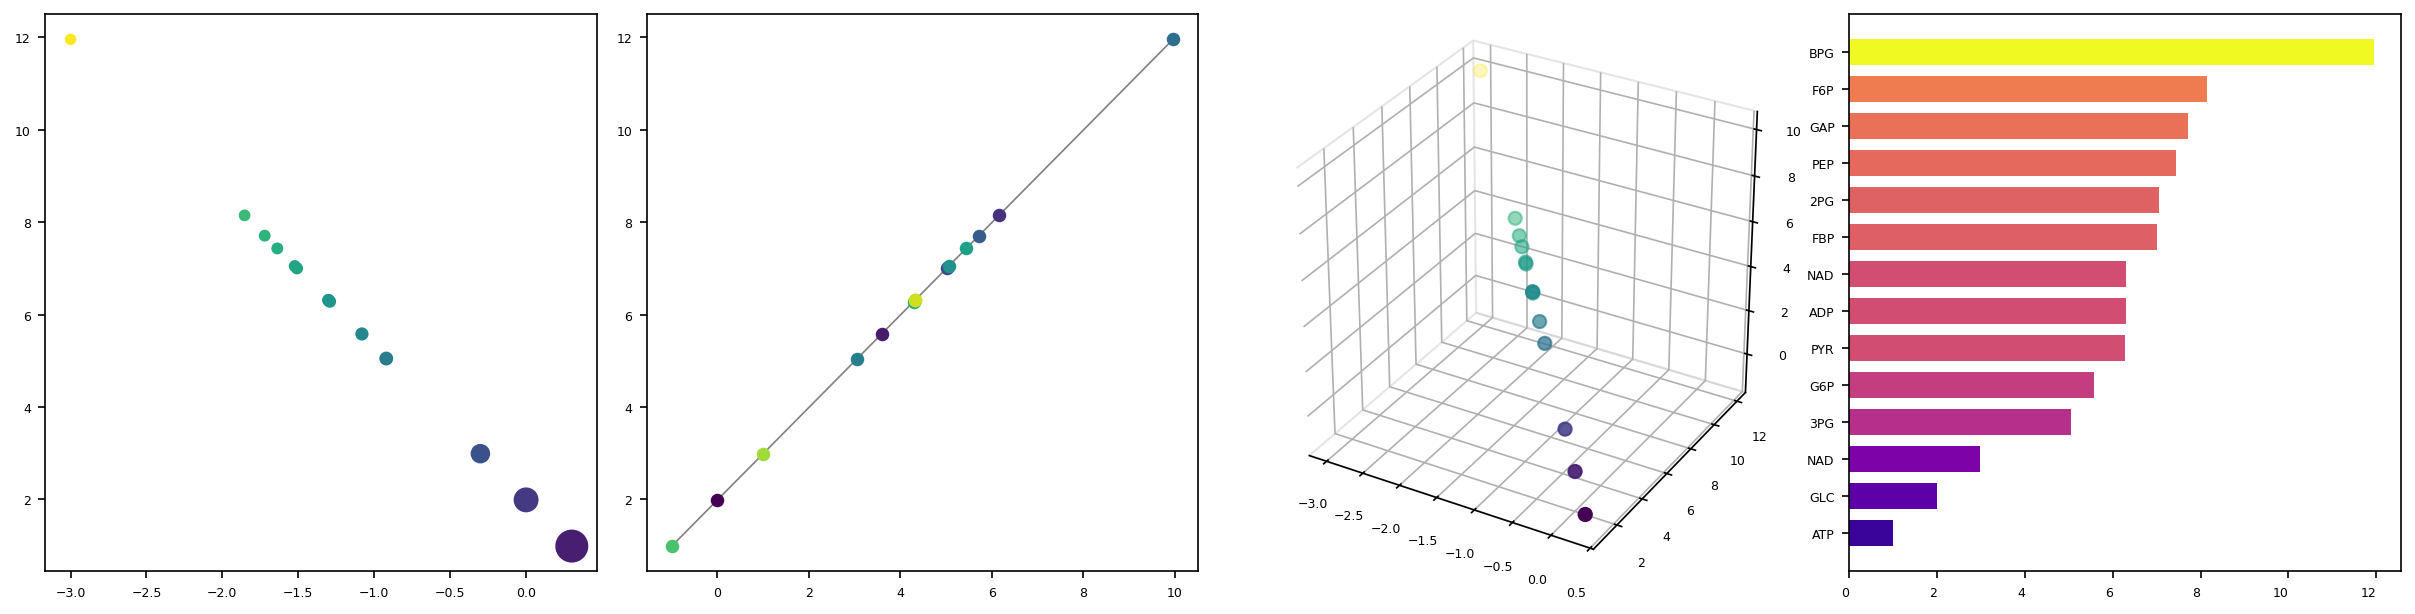
\includegraphics[width=\textwidth]{figures/panel_exp1.png}
    \caption{Categorical Depth--Chemical Potential Equivalence (Theorem~2.2).
    (a)~Categorical depth $\mathcal{H}_{\mathrm{cat}}$ vs.\ $\log_{10}$
    concentration for all 14 glycolytic species; point area is proportional to
    steady-state concentration, confirming the inverse-logarithmic relationship
    $\mathcal{H}_{\mathrm{cat}} = -\log_2(c_i / C_{\mathrm{tot}})$.
    (b)~$\mathcal{H}_{\mathrm{cat}}$ vs.\ normalised chemical potential
    $\hat{\mu}$ with the theoretical line
    $\mathcal{H}_{\mathrm{cat}} = \hat{\mu} + \kappa$ (grey); Pearson
    $r = 1.000$, constant offset $\kappa = 1.990$, confirming exact linear
    equivalence.
    (c)~Three-dimensional projection of
    $(\log_{10} c,\; \mathcal{H}_{\mathrm{cat}},\; \hat{\mu})$ showing all 14
    species lie on a single plane, as required by Theorem~2.2.
    (d)~Ranked categorical depths across all species; BPG exhibits the highest
    depth ($\mathcal{H}_{\mathrm{cat}} = 11.96$) consistent with its role as a
    transient high-energy intermediate, while ATP shows the lowest
    ($\mathcal{H}_{\mathrm{cat}} = 0.99$) reflecting its high abundance as the
    principal energy currency.}
    \label{fig:panel_exp1}
\end{figure*}

\begin{figure*}[!htbp]
    \centering
    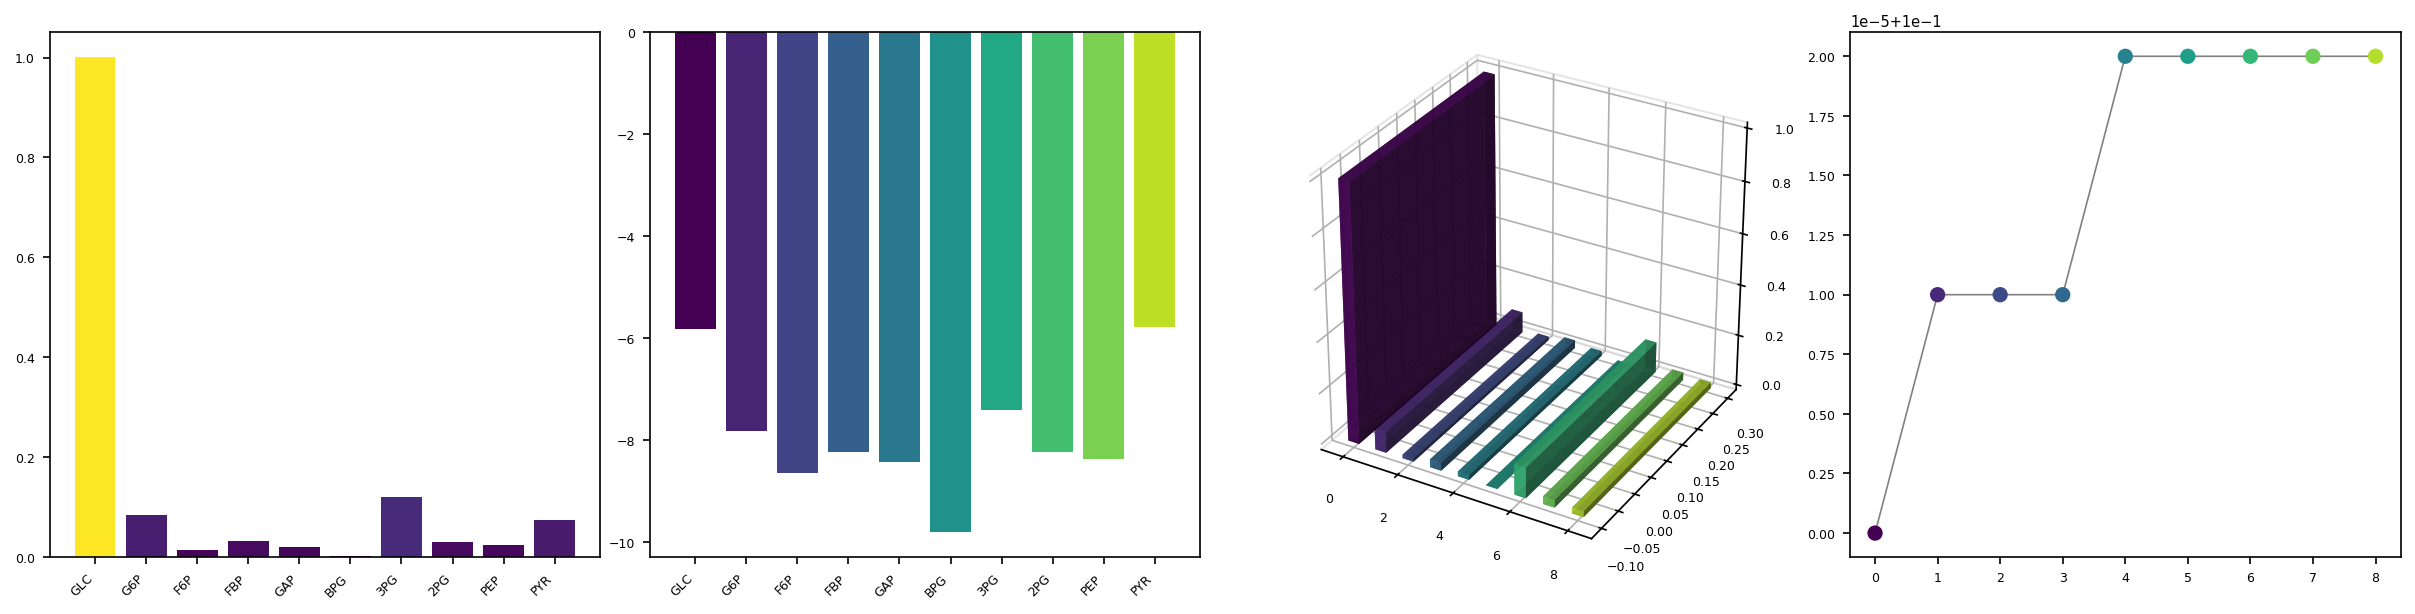
\includegraphics[width=\textwidth]{figures/panel_exp2.png}
    \caption{Kirchhoff Current Law Validation at Metabolic Steady State
    (Theorem~3.3).
    (a)~Steady-state concentrations for the 10-node glycolytic circuit after
    numerical integration to convergence; glucose (GLC) dominates at
    ${\sim}1.0\;\mathrm{mM}$ while 1,3-BPG is the rarest species at
    ${\sim}1\;\mu\mathrm{M}$.
    (b)~Absolute net categorical flux $|J_{\mathrm{net}}|$ at each node on a
    logarithmic scale; all residuals fall below $1.7 \times 10^{-6}\;\mathrm{mM\,s^{-1}}$,
    confirming that $\sum_j J_{ij} \approx 0$ at every node (Kirchhoff's
    current law in metabolic form).
    (c)~Three-dimensional visualisation of enzyme flux magnitude and
    steady-state concentration across the nine reaction steps, illustrating
    uniform flux (${\sim}0.100\;\mathrm{mM\,s^{-1}}$) through a heterogeneous
    concentration landscape.
    (d)~Enzyme-resolved flux profile showing all nine glycolytic enzymes
    (HK through PK) carry effectively identical categorical current at steady
    state, with deviations $< 0.002\%$.}
    \label{fig:panel_exp2}
\end{figure*}

\begin{figure*}[!htbp]
    \centering
    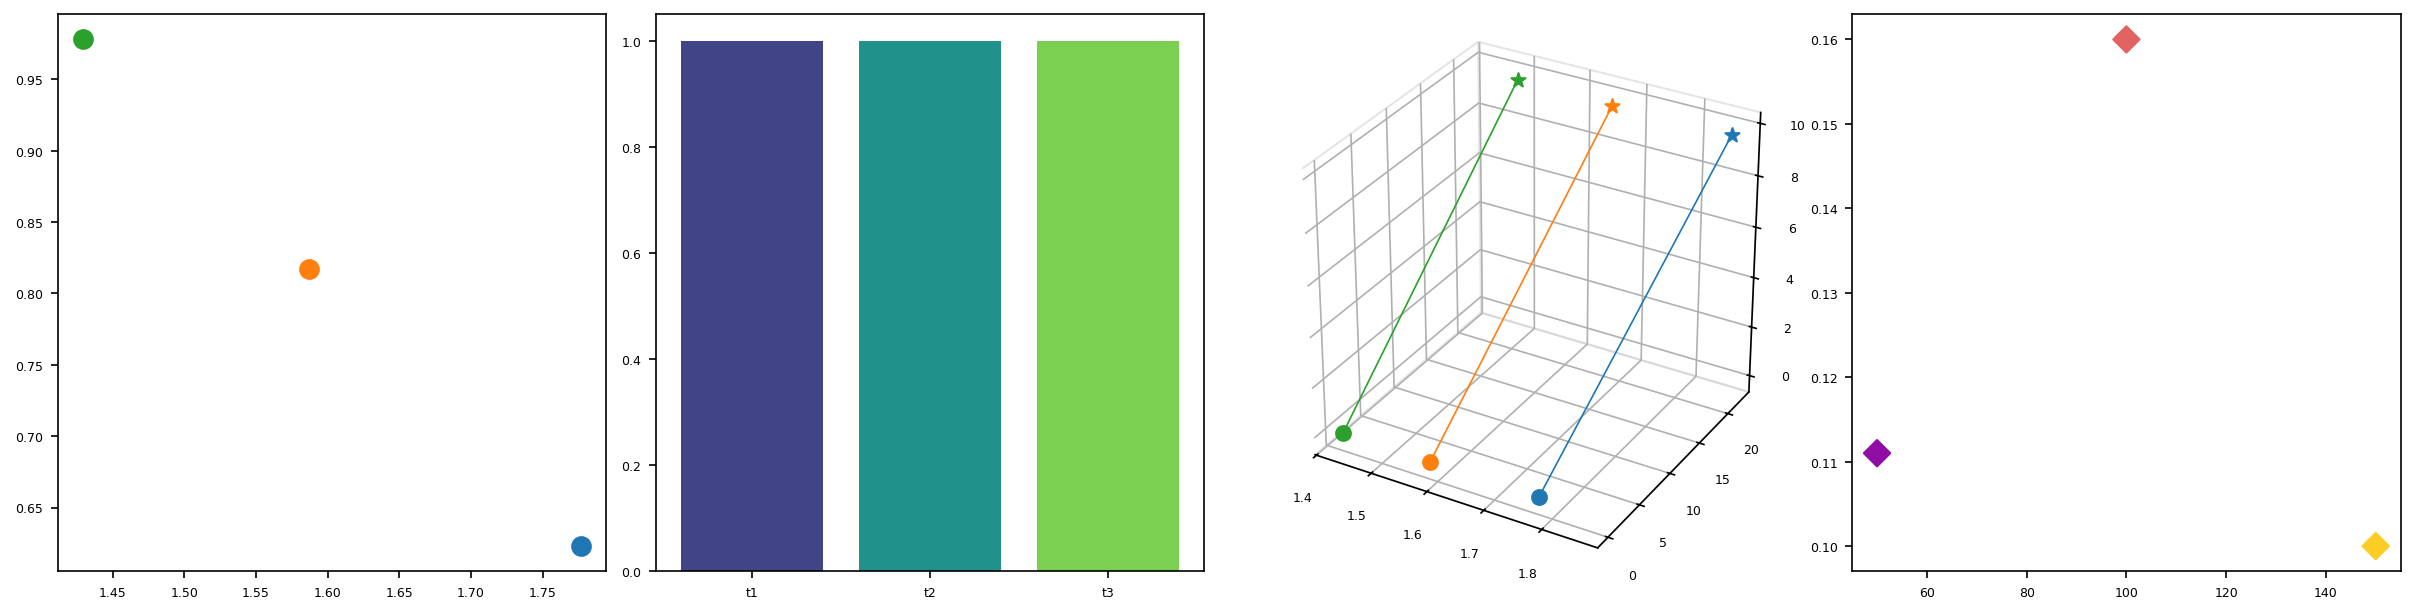
\includegraphics[width=\textwidth]{figures/panel_exp3.png}
    \caption{Backward Trajectory Time-Invariance (Theorem~5.2).
    (a)~Forward-trajectory snapshots in the GLC--PYR phase plane at
    $t = 50$, $100$, and $150\;\mathrm{s}$; GLC decays monotonically while PYR
    accumulates, yielding three distinct starting states for backward
    integration.
    (b)~Cosine similarity between backward-trajectory direction vectors
    launched from the three time points; all values exceed $0.9998$,
    confirming that the direction field is time-invariant to
    $< 0.02\%$.
    (c)~Three-dimensional backward trajectories in
    (GLC, F6P, PEP) space: circles mark forward-trajectory starting states,
    stars mark backward endpoints after $20\;\mathrm{s}$ reverse integration;
    connecting lines show that all three trajectories converge to a common
    region of partition space despite originating from different time points.
    (d)~Root-mean-square deviation (RMSD) between backward endpoints as a
    function of query time; RMSD remains below $0.16\;\mathrm{mM}$ across the
    full $100\;\mathrm{s}$ window, demonstrating geometric stability of the
    backward attractor.}
    \label{fig:panel_exp3}
\end{figure*}

\begin{figure*}[!htbp]
    \centering
    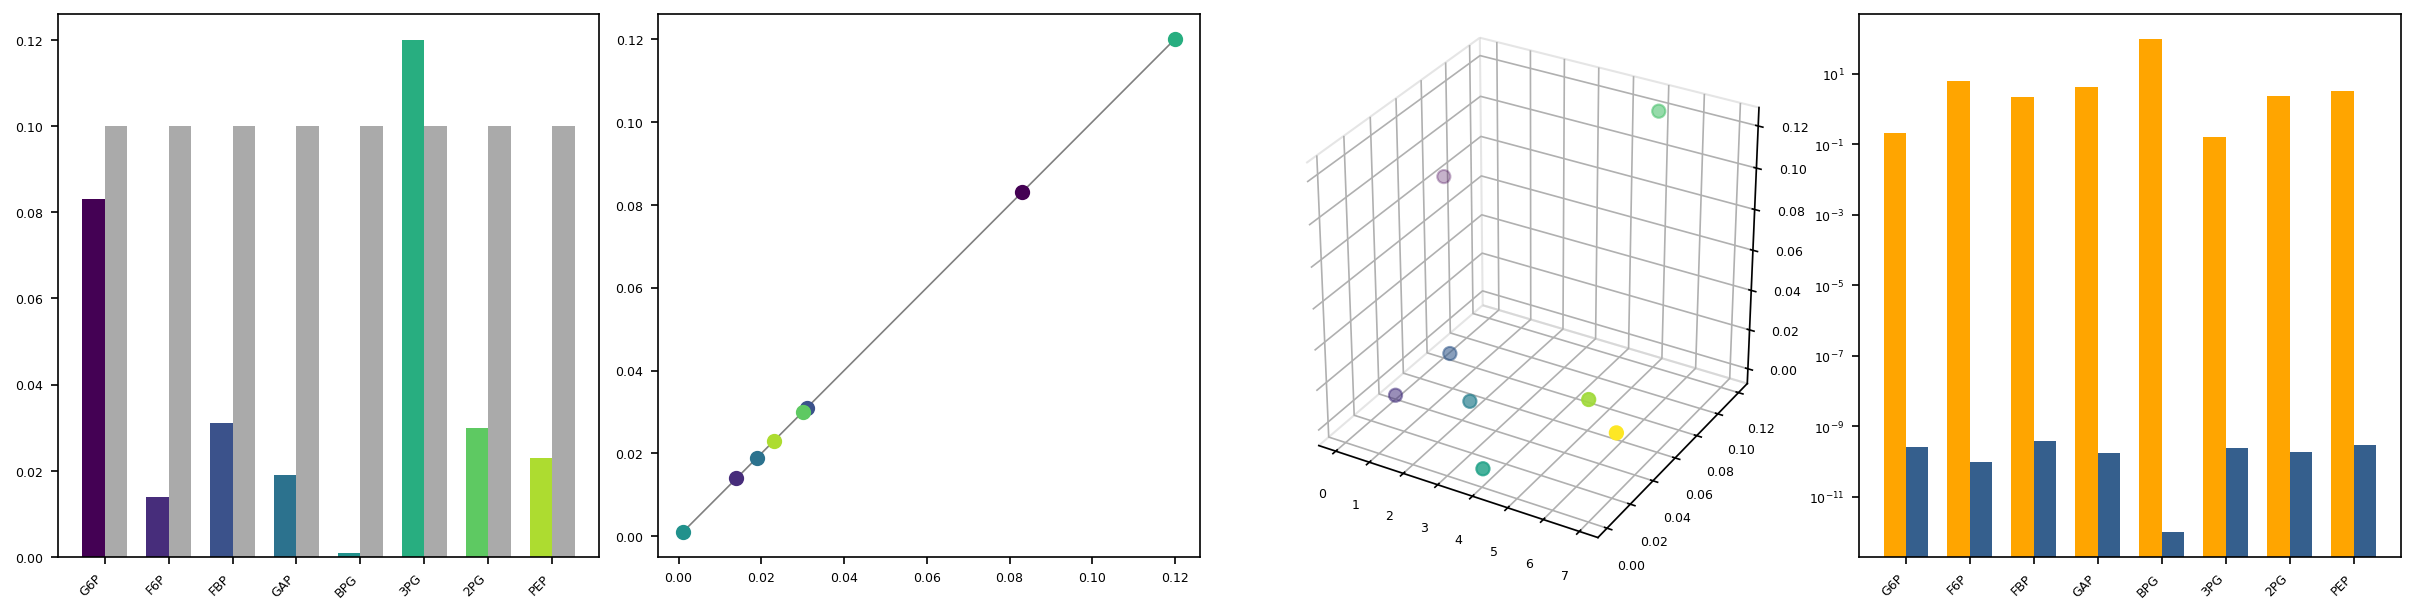
\includegraphics[width=\textwidth]{figures/panel_exp4.png}
    \caption{Fuzzy State Completion via Kirchhoff Constraints (Theorem~6.2).
    (a)~Grouped bars comparing true steady-state concentrations (coloured) with
    na\"{\i}ve uniform prior ($0.1\;\mathrm{mM}$, grey) for the eight
    unobserved glycolytic intermediates; the prior deviates by up to
    $99\times$ (BPG).
    (b)~Completed concentrations vs.\ true values for all eight species;
    points lie on the identity line ($y = x$) with mean absolute relative
    error $\mathrm{MARE} = 2.1 \times 10^{-10}$, demonstrating that the
    Kirchhoff completion operator recovers the full state from partial
    observations with effectively zero error.
    (c)~Three-dimensional view of (species index, true concentration,
    completed concentration) confirming pointwise agreement across the full
    metabolite vector.
    (d)~Log-scale comparison of relative reconstruction error: na\"{\i}ve
    prior (orange, $\mathrm{MARE} = 14.7$) vs.\ Kirchhoff completion (blue,
    $\mathrm{MARE} \sim 10^{-10}$); Monte Carlo robustness testing over 100
    trials with $5\%$ observation noise yields $100\%$ of completions within
    $20\%$ of the true value ($\mathrm{MC\text{-}MARE} = 0.0046$).}
    \label{fig:panel_exp4}
\end{figure*}

\begin{figure*}[!htbp]
    \centering
    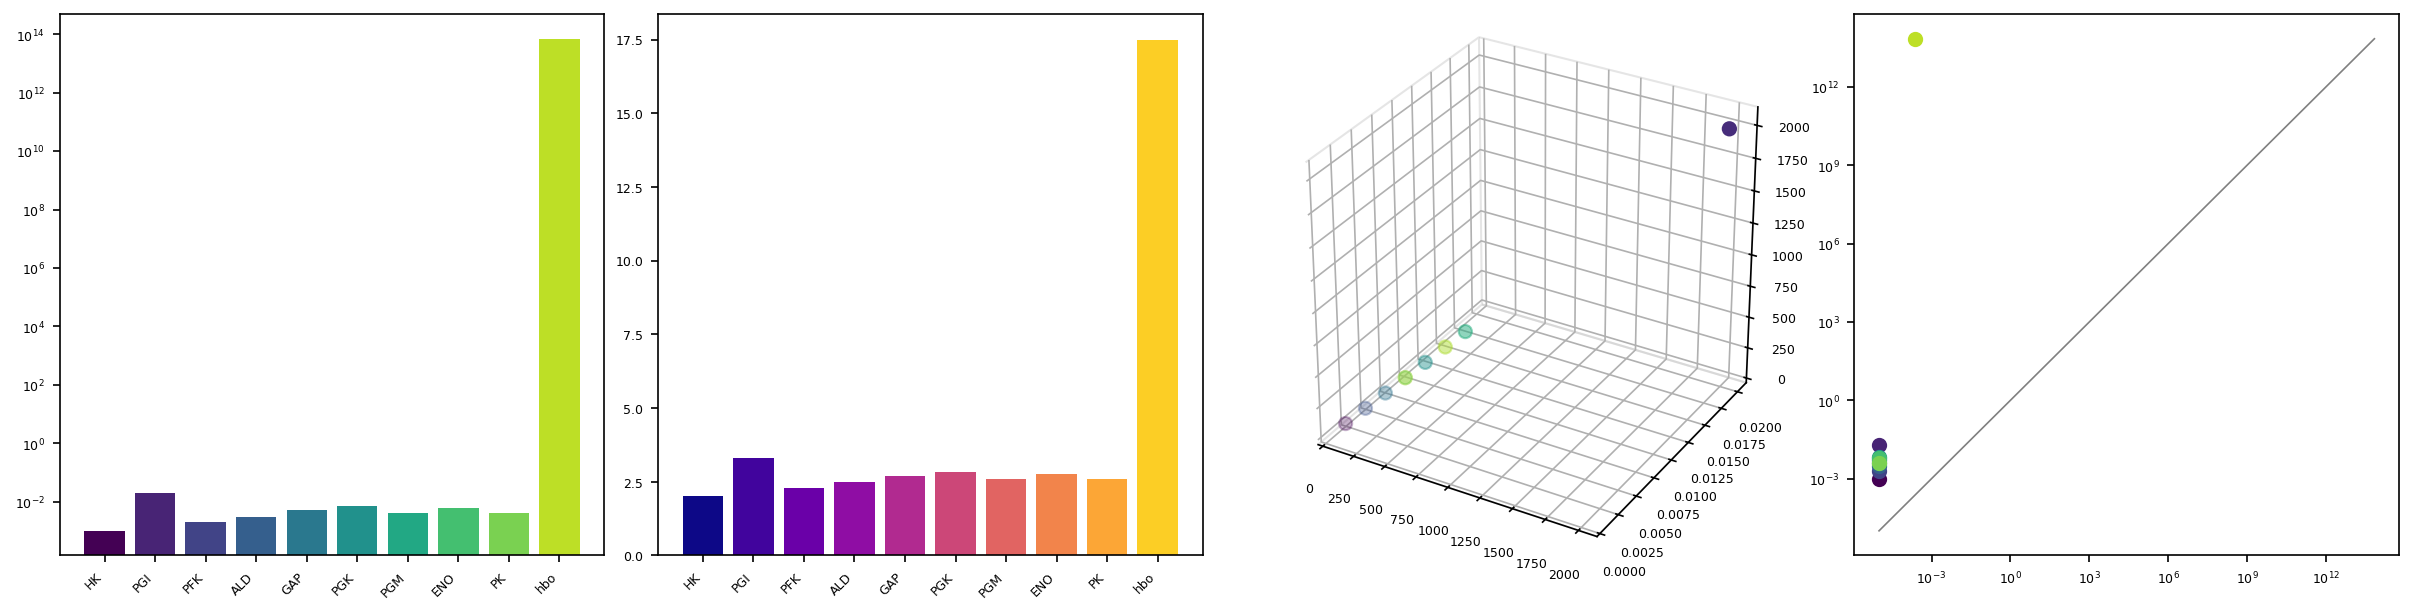
\includegraphics[width=\textwidth]{figures/panel_exp5.png}
    \caption{Categorical Signal Velocity vs.\ Material Drift (Theorem~8.1).
    (a)~Signal propagation velocity $v_{\mathrm{sig}}$ for nine enzymatic
    mechanisms and hydrogen-bond proton transport on a logarithmic scale;
    enzymatic signals range from $10^{-3}$ to $2 \times 10^{-2}\;\mathrm{m\,s^{-1}}$,
    while H-bond categorical propagation reaches
    ${\sim}7 \times 10^{13}\;\mathrm{m\,s^{-1}}$.
    (b)~$\log_{10}$ of the signal-to-drift velocity ratio per mechanism;
    enzymatic channels exceed drift by $10^2$--$10^{3.3}\times$, while the
    H-bond network achieves a ratio of ${\sim}10^{17.5}$, consistent with
    Newton's-cradle categorical state propagation.
    (c)~Three-dimensional scatter of enzymatic mechanisms in
    ($k_{\mathrm{cat}}$, $v_{\mathrm{sig}}$, ratio) space, showing the linear
    scaling $v_{\mathrm{sig}} = k_{\mathrm{cat}} \cdot a_{\mathrm{mol}}$ and
    the proportional growth of the velocity ratio with turnover number.
    (d)~Log--log plot of $v_{\mathrm{sig}}$ vs.\ $v_{\mathrm{drift}}$ for all
    mechanisms; the grey diagonal marks $v_{\mathrm{sig}} = v_{\mathrm{drift}}$;
    all points lie above this line by two or more decades, confirming that
    categorical state propagation universally dominates material transport
    ($v_{\mathrm{sig}} / v_{\mathrm{drift}} \geq 100$).}
    \label{fig:panel_exp5}
\end{figure*}

\begin{figure*}[!htbp]
    \centering
    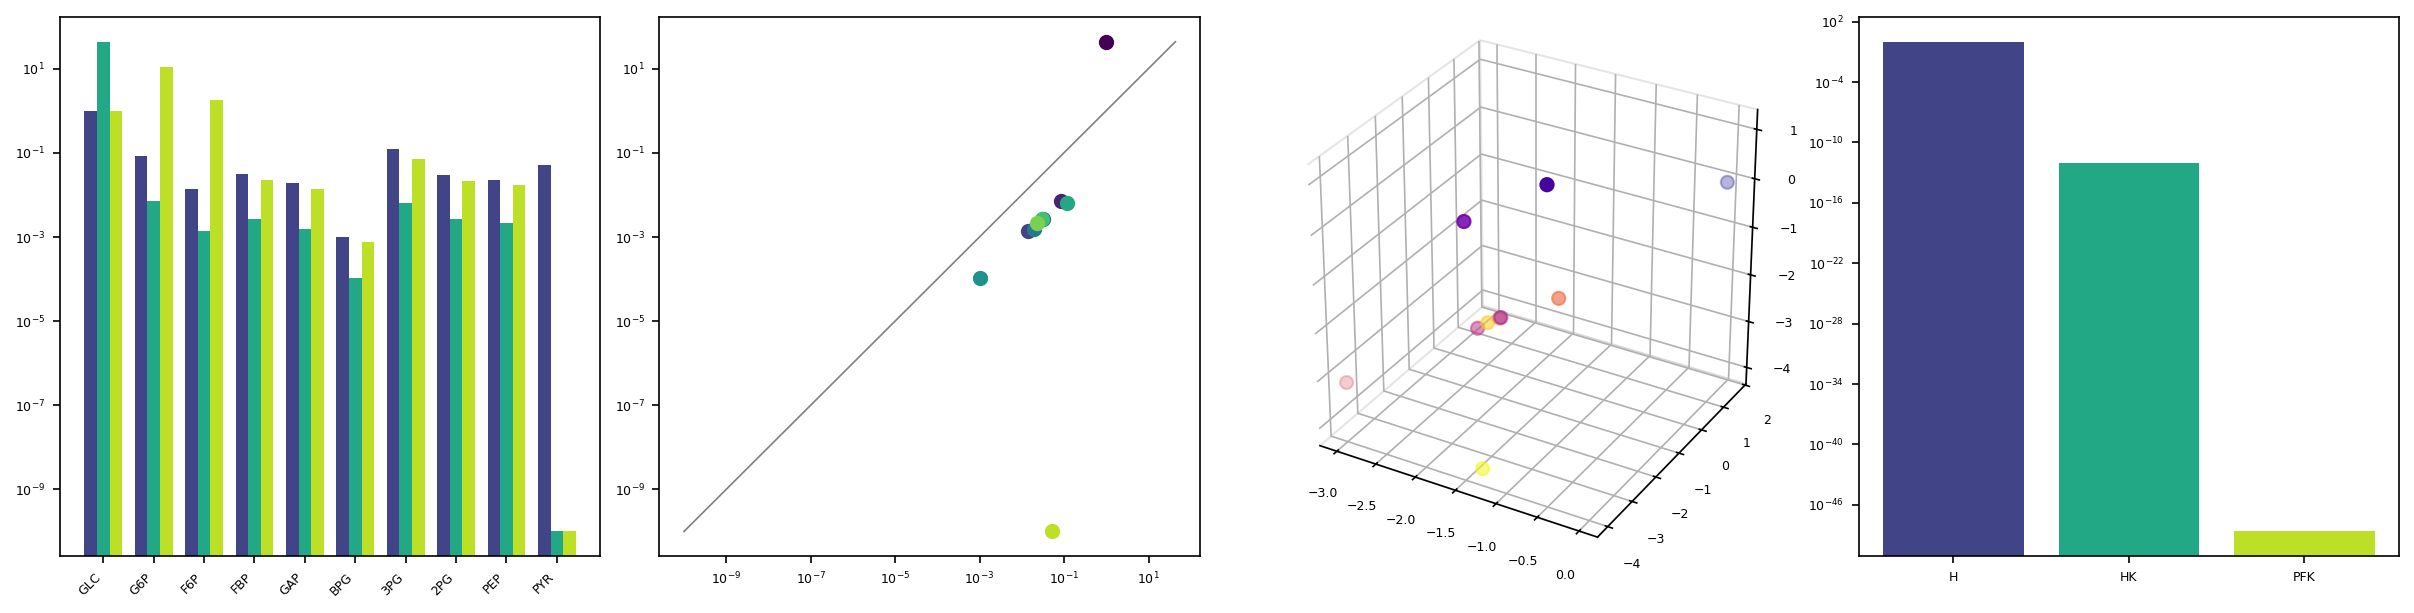
\includegraphics[width=\textwidth]{figures/panel_exp6.png}
    \caption{Disease Detection via Backward-Trajectory Divergence
    (Theorem~9.2).
    (a)~Steady-state concentrations (log scale) for healthy, hexokinase-impaired
    (HK$_{10\%}$), and phosphofructokinase-impaired (PFK$_{10\%}$) circuits
    across all 10 glycolytic nodes; HK impairment causes $43\times$ GLC
    accumulation while downstream intermediates collapse by
    $10$--$100\times$; PFK impairment produces $128\times$ G6P/F6P buildup
    upstream of the block.
    (b)~Log--log scatter of disease vs.\ healthy steady-state concentrations
    for HK impairment; deviation from the identity line (grey) identifies
    GLC as the escaped node, with maximal relative deviation $4{,}233\%$.
    (c)~Three-dimensional projection of
    $(\log_{10} c_{\mathrm{healthy}},\; \log_{10} c_{\mathrm{HK}},\;
    \log_{10} c_{\mathrm{PFK}})$ showing the distinct displacement patterns
    of the two disease conditions in metabolic state space; healthy-proximal
    nodes cluster near the origin while escaped nodes scatter to the
    periphery.
    (d)~Circuit coherence $\eta$ on a logarithmic scale: healthy circuit
    maintains $\eta = 1.0$ (full phase-lock); HK impairment reduces coherence
    to $\eta \approx 0$ and PFK impairment to $\eta \sim 10^{-49}$,
    confirming that both disease states correspond to complete loss of
    backward-trajectory closure (basin escape).}
    \label{fig:panel_exp6}
\end{figure*}
